\chapter{Phase 1 --- Modèle baseline}
\label{chap:phase1}

\section{Objectifs et cadrage}

Rappel du cadrage méthodologique (chapitre~\ref{chap:contexte}) : ce modèle est une
\textbf{référence de sanité}, pas l'objectif du projet. L'interprétabilité
(chapitres suivants, Phase 2--3) est la contribution centrale de la thèse ; le
baseline doit être ``assez bon'' et surtout \textbf{méthodologiquement sobre} --- des
choix exotiques (loss non standard, augmentation agressive, architecture
expérimentale) rendraient impossible de distinguer plus tard un vrai phénomène
d'interprétabilité d'un artefact de méthodologie.

\section{Plan : comparaison FLASH vs RSSFP au niveau modèle (pas encore implémenté)}
\label{sec:phase1-plan-flash-rssfp}

Décision de planification (11/08/2026, pas encore codée) : entraîner \textbf{3 modèles},
même architecture et mêmes hyperparamètres, pour rendre la comparaison FLASH vs RSSFP
(EDA \S\ref{sec:flash-vs-rssfp}) exploitable au niveau modèle et pas seulement au
niveau contraste brut :

\begin{itemize}[nosep]
    \item \textbf{Modèle pooled} (toutes séquences, FLASH+RSSFP+D+G) --- servira de
        base pour l'analyse d'interprétabilité des Phases 2--3.
    \item \textbf{Modèle FLASH seul} (D+G).
    \item \textbf{Modèle RSSFP seul} (D+G).
\end{itemize}

\textbf{Pourquoi pas juste évaluer le modèle pooled séparément par séquence} : un
modèle entraîné conjointement sur les deux séquences pourrait être biaisé par la
séquence au signal le plus fort (FLASH a un CNR nettement supérieur sur ASC/VSC, EDA
\S\ref{sec:flash-vs-rssfp}) --- un écart de Dice mesuré sur ce modèle unique
mélangerait ``qualité intrinsèque de la séquence'' et ``effet de l'entraînement
conjoint''. Deux modèles dédiés, à capacité égale, isolent proprement la question
``que peut apprendre ce modèle à partir de cette séquence seule''.

\textbf{Compromis assumé} : chaque modèle spécialisé n'aura accès qu'à la moitié des
données du modèle pooled (une seule paire D/G au lieu de deux) --- risque de
sur-apprentissage accru sur un dataset déjà petit (voir \S\ref{sec:phase1-augmentation},
l'augmentation de données réduit ce risque mais ne l'élimine pas). Compromis jugé
acceptable car \textbf{symétrique} entre les deux modèles spécialisés (même perte de
données des deux côtés), donc la comparaison reste valide même si les Dice absolus de
chaque modèle spécialisé seront probablement inférieurs à ceux du modèle pooled.

\todonote{Implémentation à faire : ajouter un filtre par type de séquence à
\texttt{TOSDataset} (\texttt{src/dataset.py}) et un flag \texttt{--sequence
\{all,FLASH,RSSFP\}} à \texttt{scripts/train\_phase1.py}. Utiliser la même validation
croisée \texttt{KFold} patient-level (\S split) pour chacun des 3 modèles, pas un
split unique --- d'autant plus important vu la réduction de données pour les 2
modèles spécialisés.}

\section{Architecture}

\textbf{U-Net 2D} (Ronneberger, Fischer \& Brox, 2015, \emph{MICCAI}) --- volontairement
pas état de l'art. 4 niveaux de descente/remontée, 32 canaux à la première couche
(doublés à chaque niveau), $\approx$ 7,7 millions de paramètres. Entrée : 1 canal
(image IRM en niveaux de gris, une frame à la fois) ; sortie : 7 classes (logits,
softmax appliqué dans la loss) --- fond + les 6 structures canoniques.

\textbf{Pourquoi 2D et pas 3D} : chaque frame de la séquence dynamique est traitée
indépendamment. Cohérent avec le fait que les 20 frames annotées d'une série ne sont
pas des coupes spatiales adjacentes mais des instants temporels d'une même coupe --- un
U-Net 3D supposerait une continuité spatiale entre ``slices'' qui n'existe pas ici (la
cohérence \emph{temporelle} entre frames est un axe d'analyse à part, prévu en Phase 3,
pas une hypothèse à coder en dur dans l'architecture de la Phase 1).

\section{Données et split}

\texttt{src/dataset.py} (\texttt{TOSDataset}) charge chaque frame individuellement
depuis \texttt{DATA\_processed/} (déjà aligné, N4, rééchantillonné, normalisé ---
chapitre~\ref{chap:contexte} pour la Phase 0).

\textbf{Split} : validation croisée \texttt{KFold} au niveau \textbf{patient} ($k=5$,
\texttt{src/splitting.py}), pas un split fixe train/val/test --- décision prise en
Phase 0 (\S Phase 0) vu le faible nombre de patients éligibles (13). Chaque patient
apparaît exactement une fois en validation sur l'ensemble des 5 folds. Justification
déjà développée pour la fuite de données au niveau patient : Varoquaux \& Cheplygina
(2022, \emph{npj Digital Medicine}).

\texttt{2017-110\_01-0224-V1MR} (non vérifié manuellement, outlier de barycentre
récurrent) reste forcé en train sur tous les folds (\texttt{always\_train}), jamais en
validation --- même logique de prudence que dans le split fixe précédent.

\section{Fonction de perte}
\label{sec:phase1-loss}

\textbf{Dice + Cross-Entropy pondérée}, additionnées (\texttt{src/losses.py},
\texttt{DiceCELoss}).

\begin{description}[style=nextline]
    \item[Dice loss] Milletari, Navab \& Ahmadi (2016), ``V-Net: Fully Convolutional
        Neural Networks for Volumetric Medical Image Segmentation'', \emph{3DV} ---
        papier fondateur de la Dice loss pour l'entraînement de réseaux de
        segmentation, motivé explicitement par le déséquilibre fond/premier-plan.
        Moyennée également sur les 7 classes (chaque structure pèse autant que les
        autres dans la loss, peu importe sa taille).
    \item[Cross-Entropy pondérée] Poids = fréquence inverse des pixels par classe,
        \textbf{mesurée empiriquement sur le train set} (\texttt{compute\_class\_weights}),
        pas supposée a priori. Nécessaire car la CE, contrairement au Dice, n'est pas
        normalisée par classe --- sans pondération le fond ($>$99\% des pixels)
        écraserait le gradient des structures.
    \item[Pourquoi combiner les deux] Ma et al. (2021, ``Loss odyssey in medical image
        segmentation'', \emph{Medical Image Analysis}, vol. 71) comparent 20 fonctions
        de loss sur 6 datasets publics / 10+ centres médicaux : les loss composées
        (Dice+CE) sont les plus robustes, en particulier sur des tâches à fort
        déséquilibre de classes --- exactement notre cas (ratio de taille 4,3× entre
        structures, EDA \S distribution de taille, sans compter le fond).
\end{description}

\section{Métriques d'évaluation}
\label{sec:phase1-metrics}

Toujours \textbf{par structure}, jamais un seul chiffre macro-moyenné --- les tailles
varient trop (EDA \S distribution de taille) pour qu'une moyenne globale soit
interprétable.

\begin{description}[style=nextline]
    \item[Dice] Chevauchement prédiction/vérité par classe (\texttt{src/metrics.py},
        \texttt{dice\_per\_class}). Convention standard des grands challenges de
        segmentation médicale (BraTS notamment, qui rapporte le Dice par sous-région,
        jamais un score unique).
    \item[Précision / Rappel] Ajoutés en complément (\texttt{precision\_recall\_per\_class})
        --- le Dice mélange faux positifs et faux négatifs en un seul chiffre ; savoir
        si le modèle sur- ou sous-segmente une structure donnée est cliniquement
        pertinent (sous-segmenter PB, un nerf, est plus préoccupant que le
        sur-segmenter).
    \item[Hausdorff-95] Distance de surface au 95e percentile, symétrique
        (\texttt{hausdorff95\_per\_class}), calculée via \emph{distance transform}
        (\texttt{scipy.ndimage.distance\_transform\_edt}). Métrique officielle BraTS
        aux côtés du Dice ; le 95e percentile est utilisé au lieu du Hausdorff exact
        (maximum) car ce dernier est ruiné par un seul pixel aberrant isolé.
        \textbf{Complémentaire au Dice, pas redondant} : le Dice est peu sensible à un
        petit blob isolé loin de la structure principale, alors que le Hausdorff-95 le
        détecte directement --- pertinent ici puisque l'EDA a trouvé que 34/336 couples
        structure$\times$série sont fragmentés en plusieurs composantes connexes
        (surtout K1, MSC, ASC, PB, \S composantes connexes).
        Coûteux (distance transform par image) --- calculé uniquement sur le meilleur
        checkpoint en fin d'entraînement, pas à chaque epoch.
\end{description}

\section{Détails d'implémentation}

\begin{itemize}[nosep]
    \item Optimiseur Adam, taux d'apprentissage $10^{-3}$ par défaut.
    \item Taille de batch 8, entraînement sur GPU Apple Silicon (MPS) quand disponible,
        repli CPU/CUDA sinon (\texttt{scripts/train\_phase1.py}, \texttt{get\_device}).
    \item Sélection du meilleur checkpoint par Dice moyen sur les 6 structures
        (hors fond) en validation, pas par la loss d'entraînement.
    \item Commande : \texttt{python scripts/train\_phase1.py --fold 0 --epochs 30
        --batch-size 8}.
\end{itemize}

\section{Validation du pipeline (test de fumée)}

Avant tout entraînement réel, le pipeline complet (dataset $\to$ split $\to$ modèle
$\to$ loss $\to$ métriques) a été testé de bout en bout sur 2 epochs (fold 0, 10
patients train / 3 val, 780/240 frames) --- \textbf{pour vérifier que ça tourne sans
erreur, pas pour évaluer le modèle} :

\begin{itemize}[nosep]
    \item Loss décroissante (1,58 $\to$ 1,03) et Dice moyen croissant (0,33 $\to$ 0,44)
        sur seulement 2 epochs --- signal de fonctionnement correct, pas un résultat.
    \item Hausdorff-95 testé isolément sur des cas synthétiques : prédiction parfaite
        $\to$ 0 ; décalage de 5\,px $\to$ 2,5 --- comportement attendu confirmé.
    \item \textbf{Bug trouvé et corrigé pendant l'implémentation} : quand une classe
        est absente d'un batch entier, \texttt{hausdorff95\_per\_class} renvoyait
        silencieusement 0 (division par un compteur forcé à 1) au lieu de
        \texttt{NaN} --- aurait faussement dilué la moyenne avec de faux
        ``scores parfaits''. Corrigé pour renvoyer \texttt{NaN} (exclu de la moyenne)
        dans ce cas.
\end{itemize}

\section{Augmentation de données}
\label{sec:phase1-augmentation}

Implémentée le 11/08/2026 (\texttt{src/augmentation.py}, \texttt{JointAugmentation}),
après le premier entraînement sans augmentation (\S\ref{sec:phase1-resultats}) --- ce
premier run sert justement de référence pour mesurer l'effet de l'augmentation par
comparaison directe (\S\ref{sec:phase1-comparaison-aug}).

\subsection{Transformations retenues}

Chaque transformation a sa propre probabilité d'application indépendante (convention
nnU-Net --- Isensee et al. 2021), pas un choix exclusif entre transformations.
Appliquées \textbf{uniquement au train}, jamais à la validation.

\begin{center}
\begin{tabular}{lll}
\toprule
Transformation & Paramètre & Probabilité \\
\midrule
Rotation & $\pm12°$ & 0,5 \\
Scaling & 0,9--1,1$\times$ & 0,5 (même tirage que la rotation) \\
Déformation élastique & légère ($\alpha=15$, $\sigma=4$) & 0,3 \\
Gamma (contraste) & 0,85--1,15 & 0,5 \\
Luminosité & $\times$0,9--1,1 & 0,5 \\
\bottomrule
\end{tabular}
\end{center}

Rotation et scaling appliqués identiquement à l'image (interpolation bilinéaire) et au
masque (plus-proche-voisin --- jamais d'interpolation continue sur des labels entiers,
même principe que le rééchantillonnage de Phase 0). Gamma/luminosité appliqués
uniquement à l'image (l'image étant déjà z-scorée, donc potentiellement négative, elle
est remappée temporairement en [0,1] pour que le gamma ait un sens physique, puis
reprojetée dans son échelle d'origine).

\textbf{Pas de flip horizontal} : la question de savoir si les séries D et G sont de
vraies images miroir anatomiques reste non tranchée avec l'encadrant --- l'utiliser
maintenant risquerait de fabriquer de l'anatomie irréaliste si l'hypothèse est fausse.

\subsection{Justification des paramètres, et ses limites}

Paramètres volontairement plus conservateurs que les défauts nnU-Net (rotation
$\pm30°$, scaling 0,7--1,4$\times$, vérifiés dans la documentation officielle du
dépôt) : la Phase 0 a déjà rééchantillonné toutes les séries vers un spacing physique
commun spécifiquement pour éliminer l'hétérogénéité d'échelle entre séries --- une
augmentation de scaling aussi agressive que nnU-Net réintroduirait une partie de la
variance que cette correction visait à supprimer. Le dosage léger de la déformation
élastique est motivé par un résultat de la littérature sur l'augmentation en imagerie
médicale : au-delà d'un certain seuil, la déformation élastique produit des formes
anatomiquement irréalistes --- un risque direct pour nos structures les plus fines
(ASC/VSC) et les plus fragmentées (K1/MSC, \S composantes connexes).

\textbf{Le type de chaque transformation est validé par la littérature en imagerie
médicale/IRM spécifiquement}, pas emprunté sans réflexion à la vision par ordinateur
générique : Nalepa et al. (2019, \emph{Frontiers in Computational Neuroscience},
revue sur l'augmentation pour la segmentation de tumeurs cérébrales en IRM) confirment
l'efficacité de la rotation et de la déformation élastique pour ce type de données ;
un travail sur la segmentation du plexus brachial (Wang et al., \emph{arXiv:2205.08143}
--- même structure anatomique que PB dans ce projet, en échographie) confirme que
rotation + resize + shear améliorent significativement la segmentation par rapport à
l'absence d'augmentation ($p<0{,}05$).

\textbf{Limite assumée} : les valeurs numériques exactes ($\pm12°$, $\alpha=15$,
etc.) ne sont reprises d'aucune publication précise pour ce cas d'usage (petites
structures nerveuses/vasculaires en IRM dynamique) --- c'est une adaptation
conservatrice, informée par le principe général ci-dessus mais pas calibrée
empiriquement sur une référence existante. La revue de Nalepa et al. rapporte aussi
un résultat à contre-courant du choix fait ici : combiner plusieurs techniques
d'augmentation n'améliorerait pas les résultats par rapport à une seule technique bien
choisie (brightness ou déformation élastique seules ressortent comme les plus
efficaces dans leur revue) --- hypothèse non testée ici, à garder en tête si les
résultats des prochains folds ne confirment pas le bénéfice observé
(\S\ref{sec:phase1-comparaison-aug}).

\subsection{Suivi du sur-apprentissage}

Le Dice sur un sous-échantillon fixe du train set (non augmenté, même taille que le
val set --- coût raisonnable, évite de doubler le temps d'epoch) est désormais suivi
en plus du Dice de validation à chaque epoch (\texttt{train\_diag\_loader}), pour
rendre l'écart train/val directement visible plutôt que de comparer loss train et
Dice val (deux métriques différentes, peu comparables directement).

\section{Recadrage ROI (Cropping)}
\label{sec:phase1-crop}

\subsection{Approche retenue et justification}

Nos 6 structures occupent une fraction infime de l'image (94--403\,px sur
320$\times$320 = 102\,400\,px chacune, EDA \S distribution de taille) --- traiter
l'image entière gaspille de la capacité du réseau sur du fond/anatomie non
pertinente. La pratique de référence pour ce type de problème (petite structure dans
une grande image) est le \textbf{coarse-to-fine} : un premier modèle localise
grossièrement, on recadre autour de sa prédiction (avec marge), un second modèle
affine sur ce recadrage --- utilisé pour la segmentation du pancréas (Roth et al.,
Zhu et al., Zhou et al., référence classique de ce type de problème) et intégré
nativement dans la configuration ``cascade'' de nnU-Net.

\textbf{Version allégée retenue ici} (pas le cascade complet, jugé disproportionné
pour un baseline dont l'objectif n'est pas la performance, \S Objectifs et cadrage) :
au lieu d'entraîner un modèle de localisation, un \textbf{recadrage fixe unique},
dérivé des statistiques de position des structures déjà mesurées en EDA, approxime
son rôle sans coût d'entraînement supplémentaire.

\subsection{Calcul du ROI}

\textbf{Première version} : boîte englobante (min/max en H et W) de toutes les
structures confondues sur les 51 séries à géométrie résolue, bornes robustes
(percentiles 1 et 99, pas le min/max brut, pour ne pas laisser une seule série
atypique dicter la taille du crop) $y\in[117,238]$, $x\in[44,234]$, marge de 25\,px,
arrondi /16 $\to$ \texttt{(y0=88, y1=264, x0=16, x1=256)}, 176$\times$240\,px.
Vérifiée couvrir les 51/51 séries.

\textbf{Resserrement (11/08/2026)} : mesuré après coup que 96,2\% des pixels de ce
premier crop restaient du fond (voir \S suivante) --- exploration de marges plus
fines (25/15/10/5\,px) sur les mêmes bornes percentile. \textbf{Marge=15\,px
s'est révélée non sûre} : \texttt{2017-110\_01-0223-V1MR/RSSFP D} dépasse de 2\,px
en x --- le percentile 1/99 exclut par construction 1\% des cas extrêmes, donc une
marge insuffisante par-dessus peut échouer à les couvrir malgré l'apparence de
sécurité.

\textbf{Version retenue, sûre par construction} : plutôt que percentile + marge,
\textbf{vrai min/max brut} des 51 séries ($y\in[112,239]$, $x\in[40,246]$) + marge de
10\,px, arrondi /16 :

\begin{center}
\texttt{ROI\_CROP = (y0=96, y1=256, x0=23, x1=263)} $\to$ \textbf{160$\times$240\,px}
(contre 320$\times$320, soit -63\% de surface)
\end{center}

Couvre les 51/51 séries \textbf{par construction} (la marge s'ajoute au vrai
extremum, pas à une borne déjà tronquée) --- garanti, pas seulement vérifié après
coup comme la première version. Appliqué identiquement à toutes les séries (train et
val, tous folds) --- une constante fixe, jamais apprise ni spécifique à un patient.

\textbf{Limite assumée, inchangée malgré le resserrement} : même en optimisant la
marge, le gain reste modeste (fond : 96,2\%~$\to$~95,9\%, \S suivante) --- un
recadrage fixe doit nécessairement couvrir toute la variabilité anatomique de la
population, il ne peut pas descendre beaucoup plus bas sans un vrai cascade
(recadrage individualisé par cas, \S précédente), explicitement écarté ici pour
rester proportionné à un baseline.

\textbf{Limite non résolue} : calculé uniquement sur les 51 séries à géométrie
résolue --- si les 5 séries encore exclues (\texttt{0222}$\times$4,
\texttt{0223/FLASH D}) sont un jour réintégrées après vérification manuelle, revalider
qu'elles tombent bien dans ce crop avant de les utiliser telles quelles.

\subsection{Effet mesuré}

Voir \S\ref{sec:phase1-comparaison-3way} pour la comparaison complète : gain de
vitesse net ($\approx$73--75\,s/epoch contre $\approx$140--265\,s selon les runs
précédents, mais avec des anomalies de timing plus sévères sur ce run précis), effet
mitigé sur le Dice (légèrement négatif en moyenne, mais premier gain positif sur K1
et meilleur gain sur PB), et convergence nettement plus rapide (meilleur epoch à 10
au lieu de 27) avec un plateau de validation net au-delà.

\section{Résultats}
\label{sec:phase1-resultats}

Premier entraînement réel : fold 0, 30 epochs, 10 patients train (780 frames) / 3
patients val (240 frames --- \texttt{2017-110 01-0229-V1MR}, \texttt{\_0226},
\texttt{\_0227}), lancé le 11/08/2026. Meilleur checkpoint à l'epoch 27 (Dice moyen
structures = 0,7097).

\subsection{Convergence}

\begin{center}
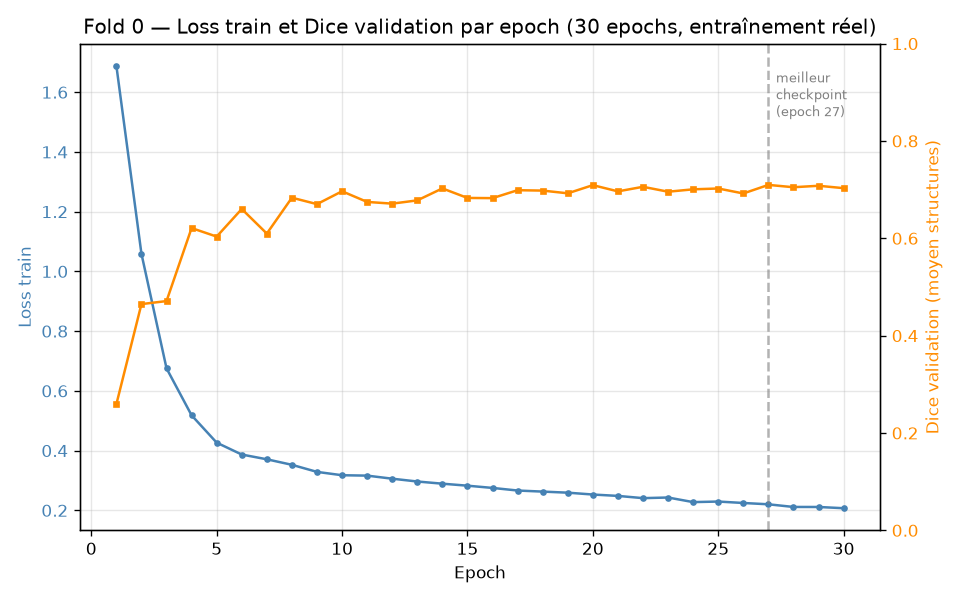
\includegraphics[width=0.75\textwidth]{figures/phase1_fold0_loss_dice_curve.png}
\end{center}

Loss décroissante de façon régulière (1,69 $\to$ 0,21), sans instabilité. Le Dice de
validation plateau à partir de l'epoch $\approx$20 autour de 0,69--0,71 --- convergence
correcte, pas de signe de divergence. \textbf{Limite de cette figure} : elle ne montre
que la loss train et le Dice val, pas le Dice train --- impossible de juger un éventuel
sur-apprentissage directement dessus. Le suivi du Dice train n'a été ajouté qu'après ce
run (\S\ref{sec:phase1-augmentation}) ; ce fold particulier ne peut donc pas être
comparé sur l'écart train/val, seulement sur ses métriques finales
(\S\ref{sec:phase1-comparaison-aug}).

\textbf{Anomalie de temps d'epoch, sans impact sur la validité} : plusieurs epochs
(4, 11, 12, 22, 27, 29) ont pris 5 à 15$\times$ plus de temps que la normale (jusqu'à
2007s contre $\approx$140s habituel), sans que la loss ou le Dice n'en soient
affectés (progression continue à travers ces epochs) --- probablement une
interférence système externe (autre processus, limitation thermique) plutôt qu'un bug
du pipeline. À surveiller si ça persiste sur les prochains entraînements.

\subsection{Résultats finaux par structure}

\begin{center}
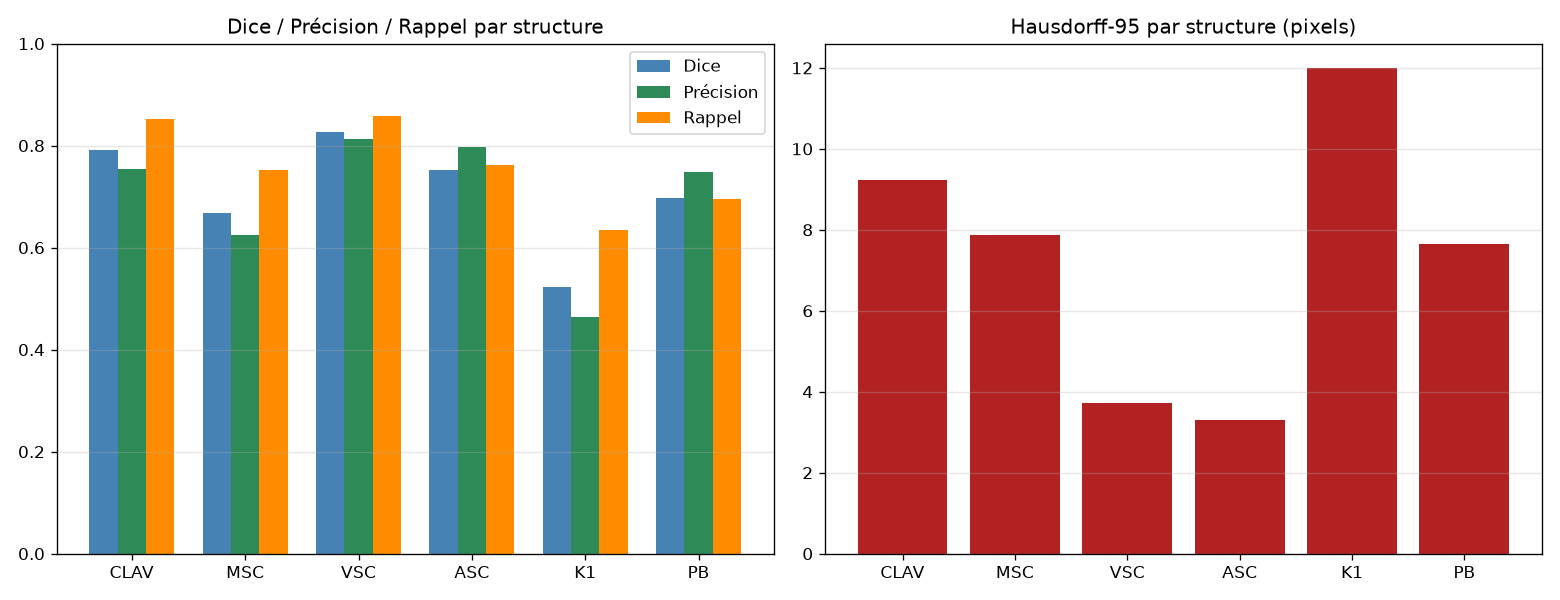
\includegraphics[width=\textwidth]{figures/phase1_fold0_final_metrics.png}
\end{center}

\begin{center}
\begin{tabular}{lrrrr}
\toprule
Structure & Dice & Précision & Rappel & Hausdorff-95 (px) \\
\midrule
fond & 0,9966 & 0,9973 & 0,9958 & 1,24 \\
CLAV & 0,7920 & 0,7545 & 0,8528 & 9,22 \\
MSC  & 0,6677 & 0,6240 & 0,7518 & 7,87 \\
VSC  & 0,8265 & 0,8129 & 0,8590 & 3,71 \\
ASC  & 0,7531 & 0,7967 & 0,7625 & 3,29 \\
K1   & 0,5224 & 0,4637 & 0,6346 & 12,00 \\
PB   & 0,6966 & 0,7484 & 0,6959 & 7,66 \\
\bottomrule
\end{tabular}
\end{center}

\textbf{Point vérifié en priorité (\S\ref{sec:phase1-loss})} : contrairement à la
crainte formulée en discutant du choix de loss, \textbf{ASC (la structure la plus
petite, EDA \S distribution de taille) ne traîne pas derrière les autres} --- Dice
0,75 et Hausdorff-95 le plus bas (3,29\,px) après VSC. La pondération de la
Cross-Entropy par fréquence inverse (poids ASC = 2,56, le plus élevé, \S précédente)
semble avoir efficacement compensé sa petite taille.

\textbf{Le vrai point faible est K1} (première côte) : Dice le plus bas (0,52),
précision la plus basse (0,46 --- beaucoup de faux positifs) et Hausdorff-95 le plus
élevé (12,00\,px). MSC est le deuxième moins bon, avec le même profil
précision~$<$~rappel (sur-segmentation plutôt que sous-segmentation).

\textbf{Cohérent avec l'EDA} : K1 et MSC étaient déjà identifiées comme les structures
les plus souvent fragmentées en plusieurs composantes connexes dans la vérité terrain
(7/56 et 9/56 séries respectivement, \S composantes connexes) --- des formes
fragmentées/complexes sont plus difficiles à apprendre pour un U-Net standard,
cohérent avec leurs moins bons scores ici. Piste à explorer si ce constat se confirme
sur d'autres folds : ce n'est pas nécessairement un problème d'architecture ou
d'hyperparamètres, mais une difficulté intrinsèque liée à la forme de ces deux
structures spécifiquement.

\subsection{Résultats qualitatifs}

\begin{center}
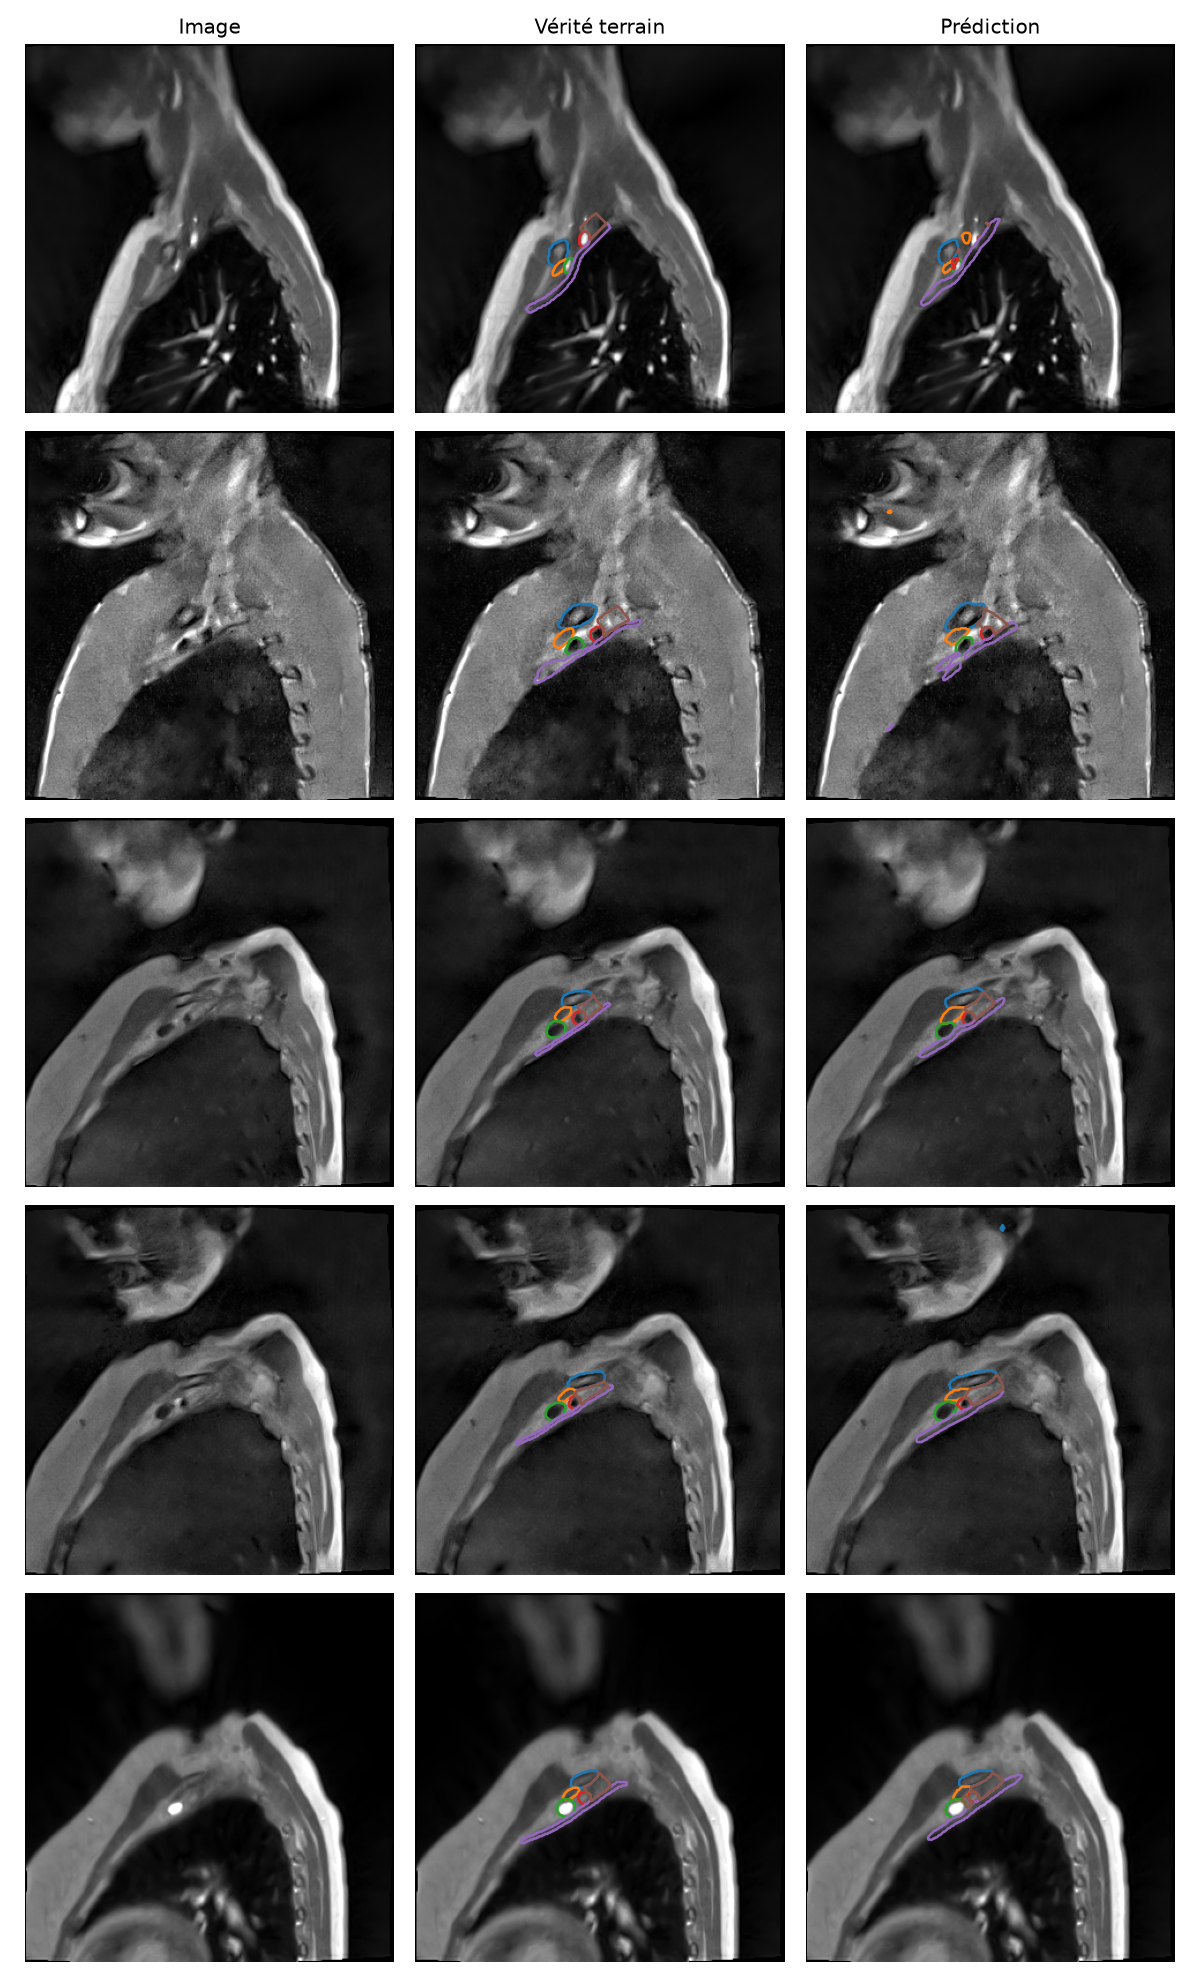
\includegraphics[width=0.5\textwidth]{figures/phase1_fold0_qualitative.png}
\end{center}

5 échantillons de validation tirés au hasard (image / contours vérité terrain /
contours prédits). Illustre concrètement deux points ci-dessus : sur un des
échantillons, le contour prédit de K1 diverge visiblement de la forme lisse de la
vérité terrain, et un \textbf{petit faux positif isolé} apparaît loin de la structure
réelle (un point de la couleur de CLAV, en haut de l'image) --- exactement le type
d'erreur que le Dice pénalise à peine mais que le Hausdorff-95 détecte fortement
(justification \S\ref{sec:phase1-metrics}), illustré ici de façon directe plutôt que
seulement statistique.

\subsection{Diagnostic de sur-apprentissage (run avec augmentation)}

\begin{center}
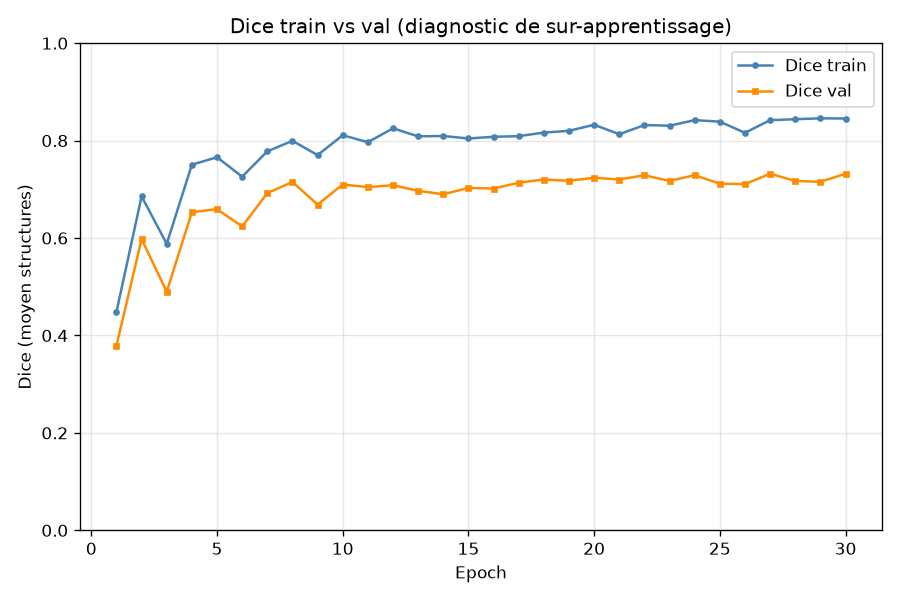
\includegraphics[width=0.7\textwidth]{figures/phase1_fold0_aug_train_val_gap.png}
\end{center}

Dice train (sous-échantillon fixe non augmenté) et Dice val suivis séparément pour la
première fois sur ce run. L'écart se creuse tôt (dès l'epoch $\approx$5) et se
stabilise ensuite autour de 0,10--0,13 (train $\approx$0,84--0,85, val
$\approx$0,71--0,73) plutôt que de continuer à s'élargir jusqu'à l'epoch 30 --- un
écart modéré et stable, pas une divergence qui s'aggrave. Signal plutôt rassurant,
mais un écart persiste malgré l'augmentation : cohérent avec le fait qu'elle a
amélioré certaines métriques (Hausdorff CLAV/MSC) sans les résoudre toutes (K1
inchangé, \S\ref{sec:phase1-comparaison-aug}).

\subsection{Évolution du Dice par structure (run avec augmentation)}

\begin{center}
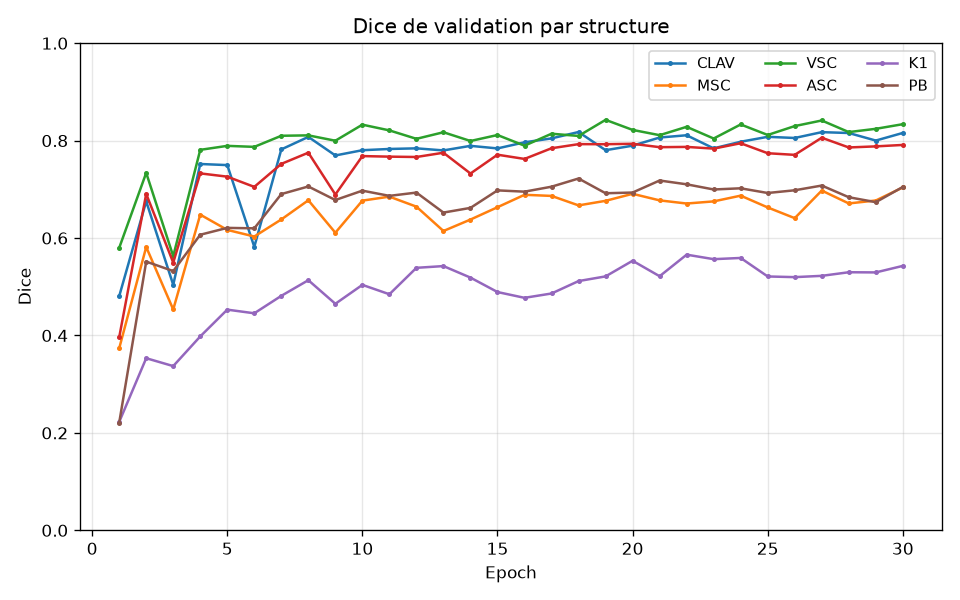
\includegraphics[width=0.75\textwidth]{figures/phase1_fold0_aug_dice_curve.png}
\end{center}

K1 (violet) est visiblement et systématiquement la courbe la plus basse \textbf{sur
l'ensemble de l'entraînement}, pas seulement au dernier epoch --- separée des 5
autres structures dès l'epoch $\approx$5 et ne les rejoint jamais. Confirme que sa
faiblesse est structurelle et présente tout du long, pas un accident de fin
d'entraînement.

\begin{center}
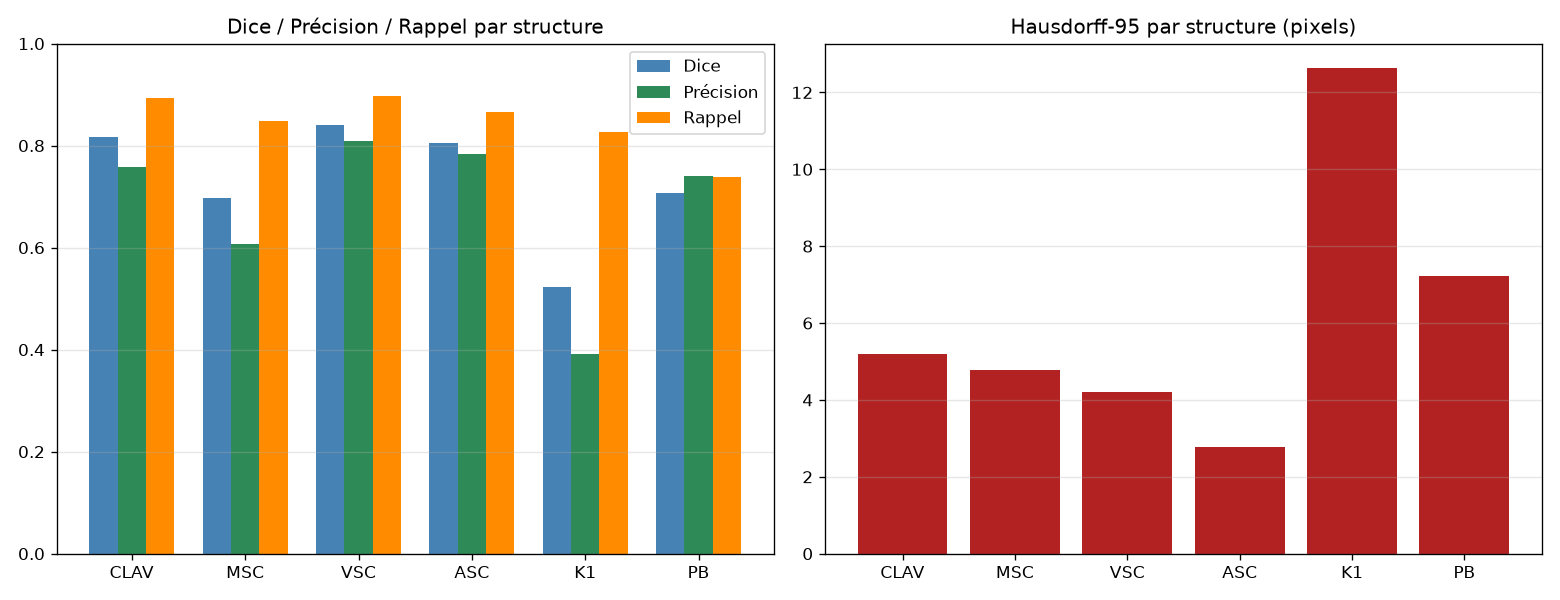
\includegraphics[width=\textwidth]{figures/phase1_fold0_aug_final_metrics.png}
\end{center}

Version graphique de la table \S\ref{sec:phase1-comparaison-aug} --- Précision de K1
(0,39) nettement en dessous de son Rappel (0,83), le plus grand écart des 6
structures : confirme visuellement la sur-segmentation caractéristique de K1.

\subsection{Résultats qualitatifs (run avec augmentation)}

\begin{center}
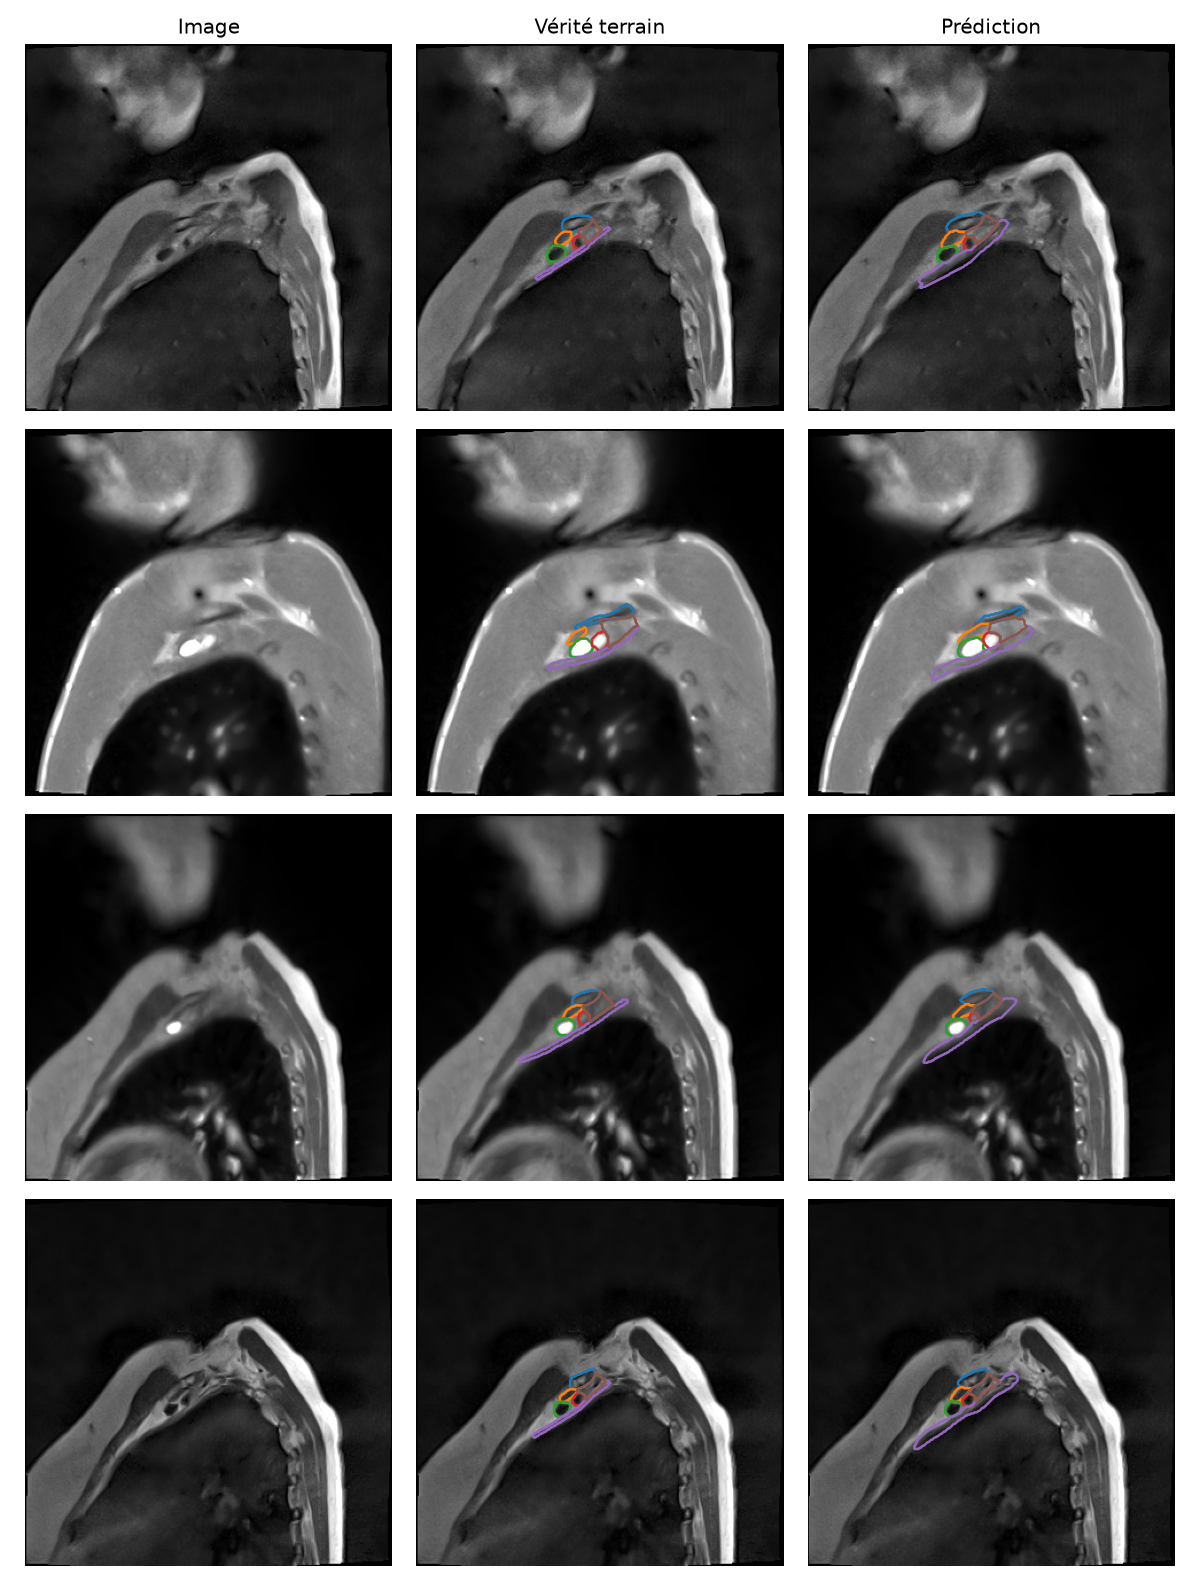
\includegraphics[width=0.5\textwidth]{figures/phase1_fold0_aug_qualitative.png}
\end{center}

4 échantillons de validation tirés au hasard (graine différente de la figure
équivalente sans augmentation, \S\ref{sec:phase1-resultats} --- donc pas une
comparaison appariée sur les mêmes frames). Aucun faux positif isolé loin de la
structure réelle n'est visible sur ces 4 échantillons, contrairement à la figure
sans augmentation --- cohérent avec l'amélioration du Hausdorff-95 sur CLAV/MSC
(\S\ref{sec:phase1-comparaison-aug}), sans que ces 4 échantillons seuls ne le
prouvent formellement.

\subsection{Comparaison avec / sans augmentation}
\label{sec:phase1-comparaison-aug}

Même fold (mêmes patients train/val), même architecture, mêmes hyperparamètres ---
seule différence : augmentation activée ou non
(\S\ref{sec:phase1-augmentation}). Comparaison contrôlée, pas juste un second run
isolé.

\begin{center}
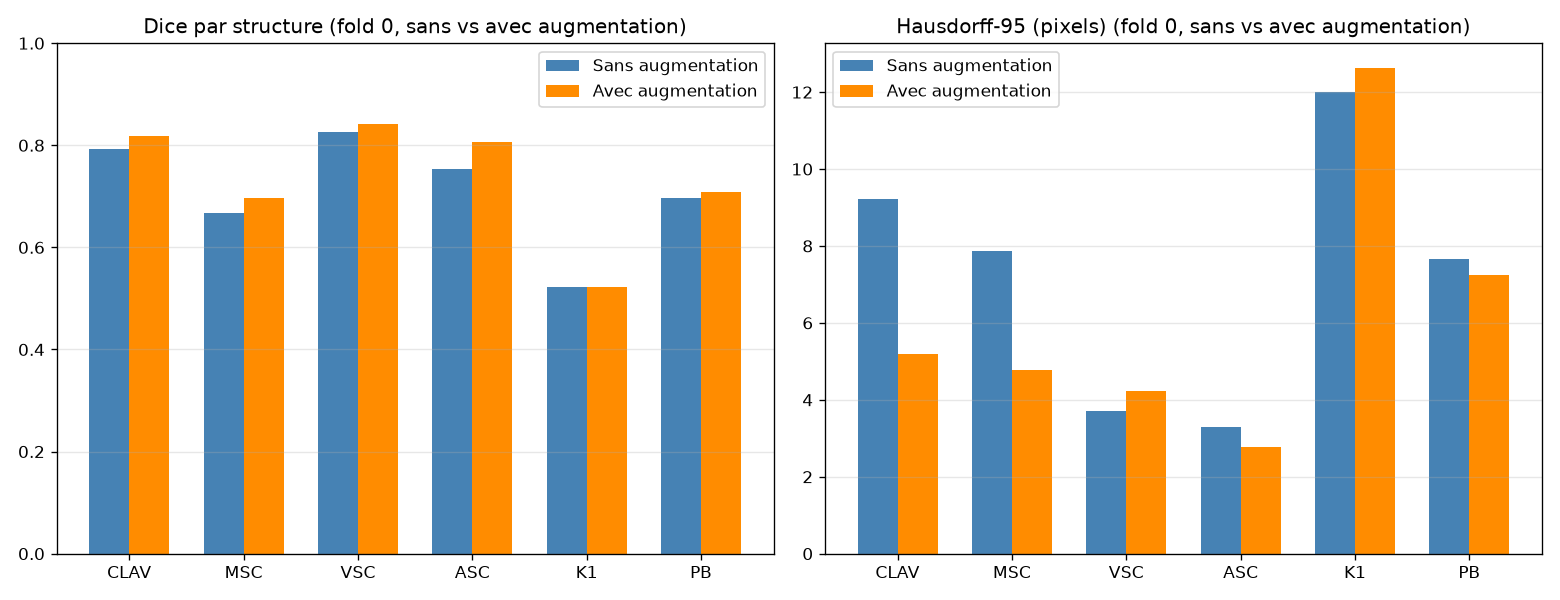
\includegraphics[width=\textwidth]{figures/phase1_fold0_aug_vs_noaug.png}
\end{center}

\begin{center}
\begin{tabular}{lrrrr}
\toprule
Structure & Dice sans aug. & Dice avec aug. & HD95 sans aug. (px) & HD95 avec aug. (px) \\
\midrule
CLAV & 0,7920 & 0,8174 (+0,025) & 9,22 & \textbf{5,20 (-44\%)} \\
MSC  & 0,6677 & 0,6975 (+0,030) & 7,87 & \textbf{4,78 (-39\%)} \\
VSC  & 0,8265 & 0,8413 (+0,015) & 3,71 & 4,22 (+0,51) \\
ASC  & 0,7531 & 0,8059 (+0,053) & 3,29 & 2,78 (mieux) \\
K1   & 0,5224 & 0,5224 (inchangé) & 12,00 & 12,64 (légèrement pire) \\
PB   & 0,6966 & 0,7078 (+0,011) & 7,66 & 7,24 (mieux) \\
\midrule
Moyenne (structures) & 0,7097 & \textbf{0,7321 (+0,022)} & --- & --- \\
\bottomrule
\end{tabular}
\end{center}

\textbf{L'effet le plus net n'est pas sur le Dice moyen (+0,022, modeste) mais sur le
Hausdorff-95 de CLAV et MSC} (-44\% et -39\%) --- cohérent avec l'hypothèse formulée en
\S\ref{sec:phase1-augmentation} : l'augmentation réduit les faux positifs isolés loin
de la structure (visibles dans la figure qualitative du run sans augmentation,
\S\ref{sec:phase1-resultats}), exactement le type d'erreur que le Dice ignore mais que
le Hausdorff-95 détecte fortement.

\textbf{K1 reste le point faible, quasiment inchangé.} Précision en baisse (0,46
$\to$ 0,39), rappel en hausse (0,63 $\to$ 0,83) --- le modèle sur-segmente encore
davantage K1 avec l'augmentation, pas moins. Ça suggère que la difficulté sur K1
n'est \textbf{pas} un problème de sur-apprentissage que l'augmentation seule peut
résoudre, mais quelque chose de plus structurel (forme fragmentée intrinsèquement
difficile, EDA \S composantes connexes, ou confusion avec une zone d'intensité
voisine) --- testé ci-après avec le recadrage ROI (\S\ref{sec:phase1-crop}).

\textbf{Limite déjà notée} : pas de comparaison possible sur l'écart train/val entre
les deux runs, le suivi du Dice train n'existant pas encore lors du run sans
augmentation.

\subsection{Comparaison à trois : sans aug/crop, avec aug, avec aug + crop}
\label{sec:phase1-comparaison-3way}

Même fold, même architecture, mêmes hyperparamètres pour les 3 runs --- seule
différence : augmentation et/ou recadrage ROI (\S\ref{sec:phase1-crop}) activés ou
non.

\begin{center}
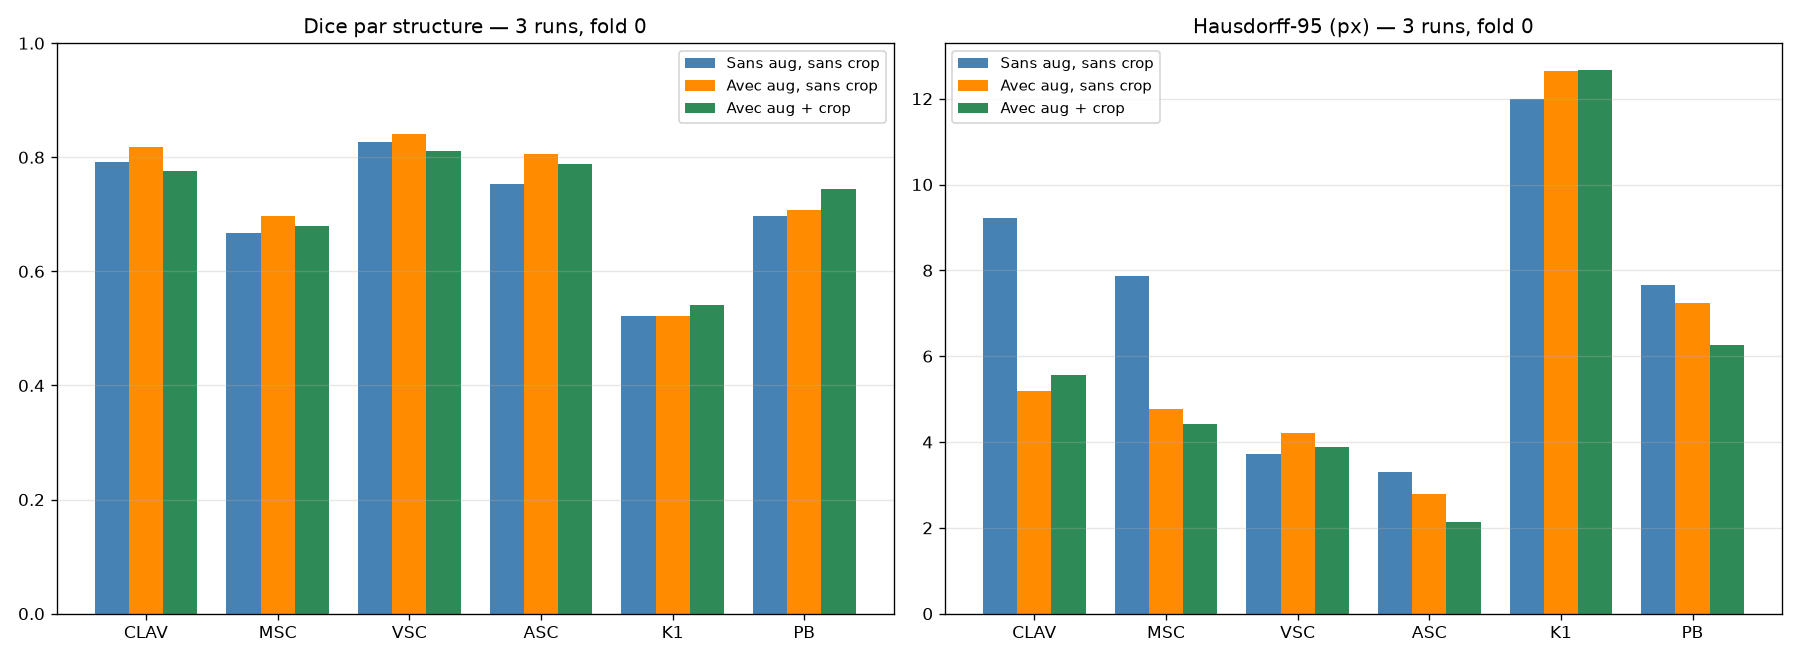
\includegraphics[width=\textwidth]{figures/phase1_fold0_3way_comparison.png}
\end{center}

\begin{center}
\begin{tabular}{lrrr}
\toprule
Structure & Dice sans aug/crop & Dice avec aug & Dice avec aug+crop \\
\midrule
CLAV & 0,7920 & 0,8174 & 0,7761 (pire) \\
MSC  & 0,6677 & 0,6975 & 0,6797 (pire) \\
VSC  & 0,8265 & 0,8413 & 0,8110 (pire) \\
ASC  & 0,7531 & 0,8059 & 0,7885 (pire) \\
K1   & 0,5224 & 0,5224 & \textbf{0,5417 (premier mouvement positif)} \\
PB   & 0,6966 & 0,7078 & \textbf{0,7444 (meilleur gain)} \\
\midrule
Moyenne & 0,7097 & 0,7321 & 0,7236 (légèrement pire que aug seule) \\
\bottomrule
\end{tabular}
\end{center}

\textbf{Le crop n'apporte pas le gain de Dice espéré} : moyenne légèrement inférieure
au run avec augmentation seule. Il aide enfin K1 (premier mouvement positif sur les 3
runs, même si K1 reste la structure la plus faible) et améliore nettement PB, mais
coûte un peu sur CLAV/VSC/ASC (qui étaient déjà les meilleures structures).

\textbf{Résultat le plus significatif : pas le Dice, mais la vitesse de
convergence.} Le meilleur checkpoint tombe à l'\textbf{epoch 10}, contre 27 pour les
deux runs précédents.

\begin{center}
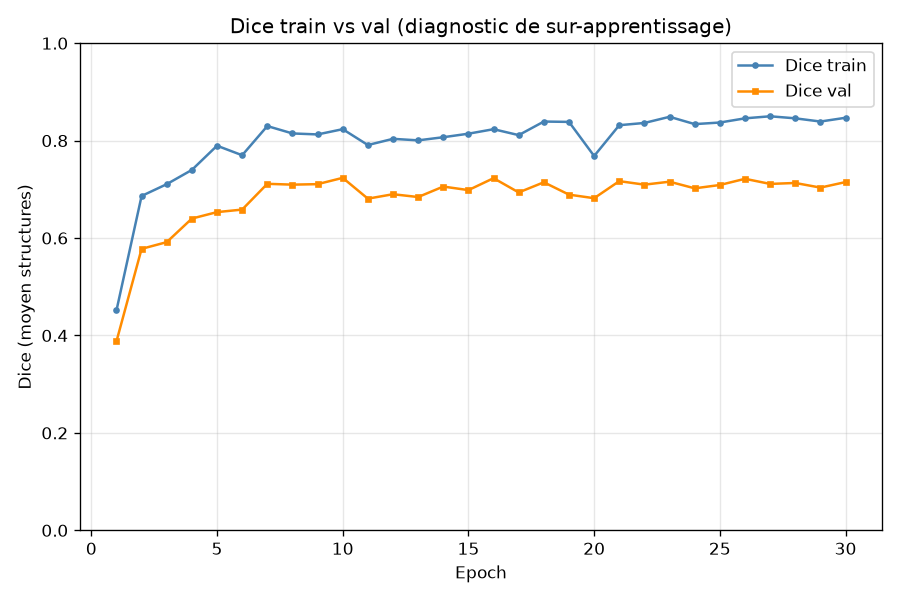
\includegraphics[width=0.7\textwidth]{figures/phase1_fold0_aug_crop_train_val_gap.png}
\end{center}

Le Dice train continue de grimper jusqu'à $\approx$0,85 tandis que le \textbf{Dice
val plateau dès l'epoch $\approx$10 et n'en bouge quasiment plus} (0,68--0,72)
jusqu'à l'epoch 30 --- sur-apprentissage plus net et plus précoce qu'avec
l'augmentation seule (\S\ref{sec:phase1-augmentation}). Interprétation : le crop
concentre le signal utile (moins de pixels par epoch), donc le modèle atteint son
plafond de généralisation plus vite, mais ce plafond n'est pas plus haut ---
continuer au-delà de l'epoch $\approx$10--15 n'apporte rien en validation.
\textbf{Recommandation pratique} : avec le crop actif, réduire le nombre d'epochs
(15 plutôt que 30) plutôt que de garder la même durée d'entraînement que sans crop.

\begin{center}
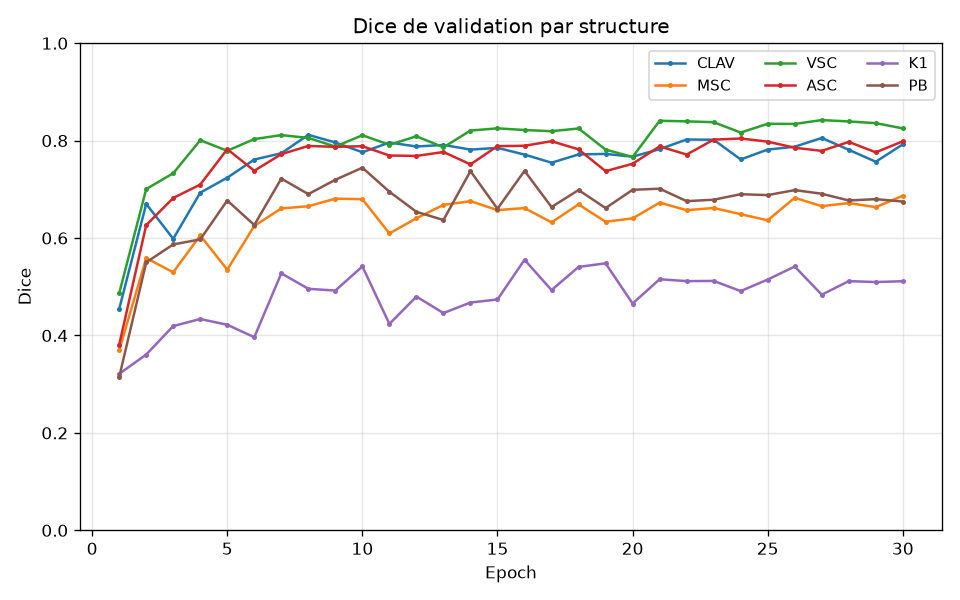
\includegraphics[width=0.75\textwidth]{figures/phase1_fold0_aug_crop_dice_curve.png}
\end{center}

Même signature qu'avec l'augmentation seule : K1 (violet) reste isolée en dessous des
5 autres structures sur tout l'entraînement, confirmant que le crop ne résout pas non
plus sa faiblesse structurelle malgré le gain ponctuel en Dice final
(\S\ref{sec:phase1-comparaison-3way}).

\begin{center}
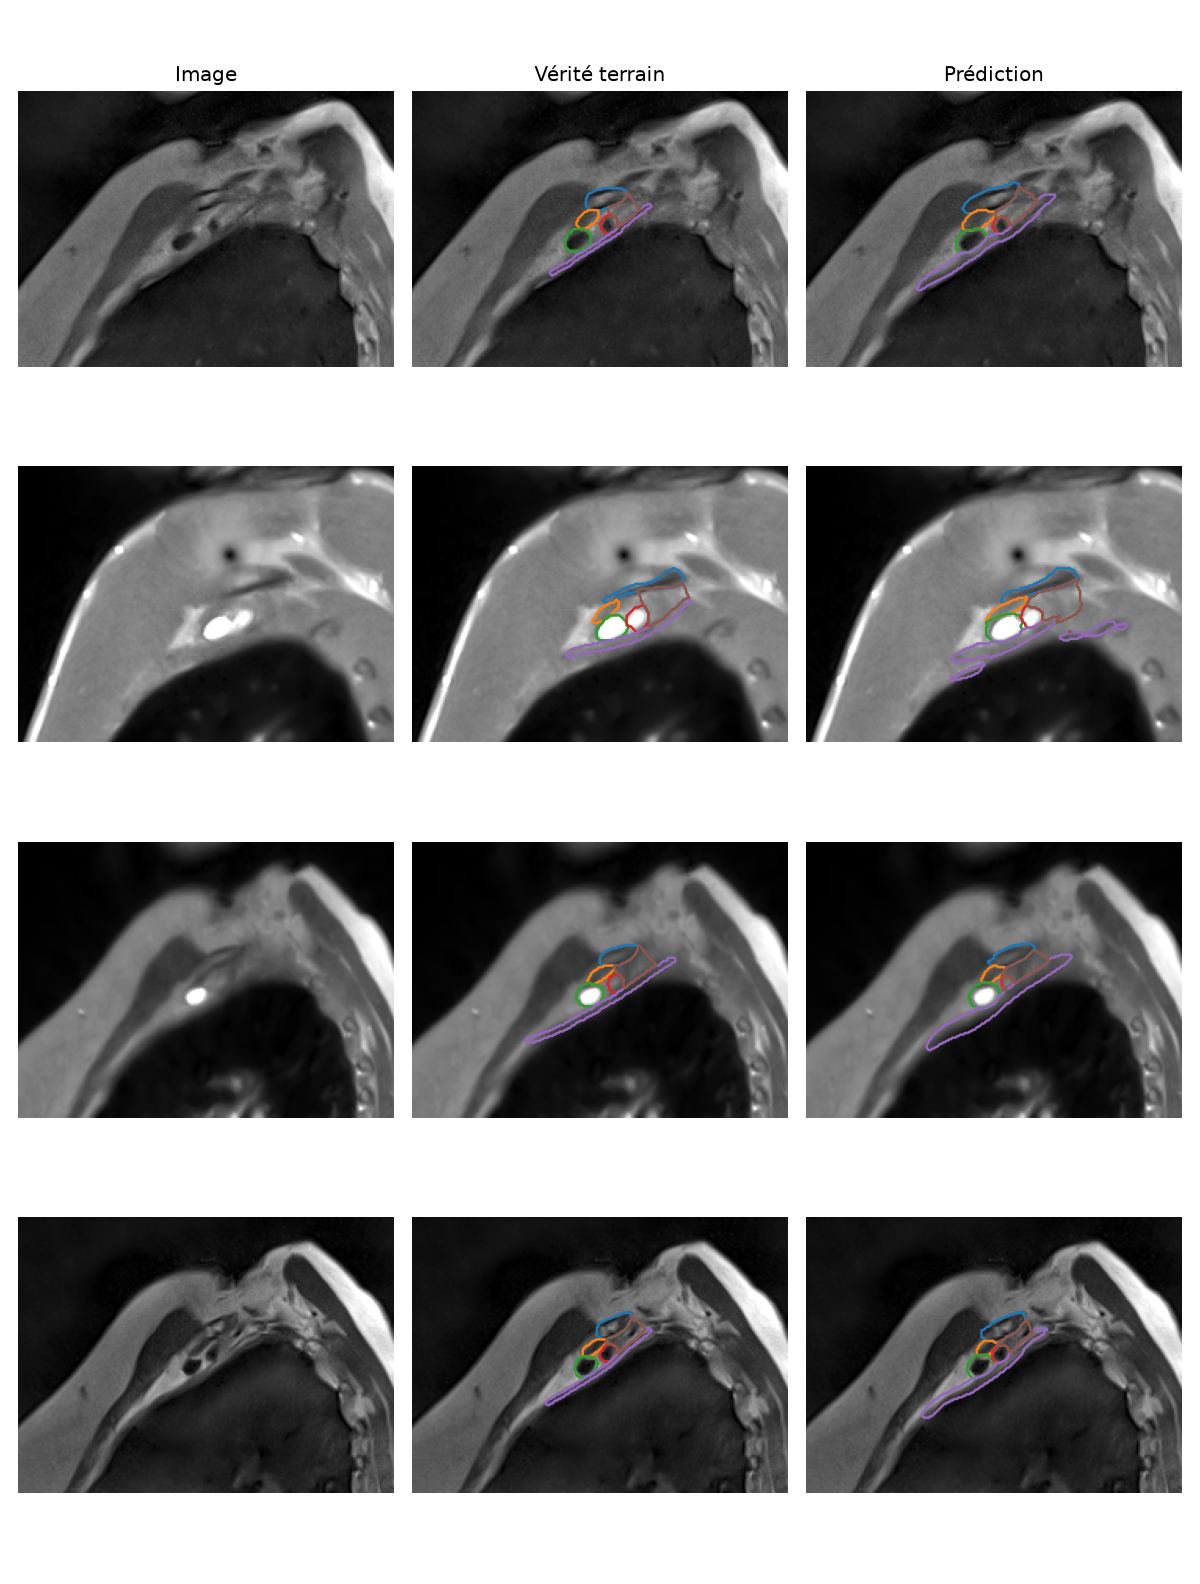
\includegraphics[width=0.55\textwidth]{figures/phase1_fold0_aug_crop_qualitative.png}
\end{center}

4 échantillons de validation (recadrés au ROI, donc cadrage différent des figures
précédentes). \textbf{Sur le 2e échantillon, le contour prédit de K1 (violet)
présente une coupure visible} --- il se scinde en deux segments disjoints alors que
la vérité terrain trace une ligne continue. Illustration directe, sur un cas concret,
de la fragmentation structurelle de K1 déjà quantifiée en EDA (\S composantes
connexes) et désormais reproduite par le modèle lui-même, pas seulement présente
dans les annotations.

\textbf{Anomalie de temps d'epoch nettement plus sévère sur ce run} : plusieurs
epochs ont pris jusqu'à 1394s contre $\approx$73--75s habituel (crop actif) ---
jusqu'à 19$\times$ plus lent, contre 5--15$\times$ sur les runs précédents. À
surveiller de près : ça commence à dépasser la simple interférence système ponctuelle
déjà notée, sans toutefois avoir affecté la validité de la progression loss/Dice.

\todonote{Une fois plusieurs folds entraînés, rapporter le Dice moyen $\pm$
écart-type inter-fold par structure (validation croisée), pas seulement ce fold
isolé --- vérifier en particulier si K1 reste systématiquement la structure la plus
faible sur les 5 folds. Décider de la configuration finale (aug seule vs aug+crop)
avant de lancer les folds restants --- si le gain de vitesse du crop est confirmé
stable (anomalie de timing à éclaircir d'abord), aug+crop avec un nombre d'epochs
réduit (15) pourrait être le meilleur compromis vitesse/qualité.}

\section{Validation croisée --- fold 1 et complément fold 0}
\label{sec:phase1-fold1}

Suite directe du todo ci-dessus : deuxième fold entraîné (12--13/08/2026) pour
commencer à distinguer un effet réel d'un artefact du split fold 0. Toutes les
combinaisons augmentation/crop n'ont pas encore été couvertes sur les deux folds
--- état exact ci-dessous.

\subsection{Runs effectués}

\begin{center}
\begin{tabular}{llrrrl}
\toprule
Fold & Config & Epochs & Meilleur epoch & Dice moyen & Anomalie timing \\
\midrule
0 & sans aug, sans crop (run initial) & 30 & 27 & 0,7097 & modérée (5--15$\times$) \\
0 & avec aug, sans crop & 30 & --- & 0,7321 & --- \\
0 & avec aug + crop & 30 & 10 & 0,7236 & sévère (jusqu'à 19$\times$) \\
0 & sans aug, sans crop (répétition, 20 epochs) & 20 & 17 & 0,7013 & modérée (jusqu'à 27$\times$, 1 epoch) \\
1 & avec aug + crop & 20 & 17 & 0,7434 & aucune notable \\
1 & sans aug + crop & 20 & 20 & 0,7585 & \textbf{extrême ($\approx$13h de run)} \\
1 & sans aug, sans crop & 20 & 16 & \textbf{0,7593} & modérée (jusqu'à 8$\times$) \\
1 & avec aug, sans crop & 20 & 17 & 0,7401 & sévère (plusieurs epochs $>$2000s) \\
0 & sans aug + crop & 20 & 17 & 0,7187 & \textbf{extrême ($\approx$12,6h de run)} \\
\bottomrule
\end{tabular}
\end{center}

\textbf{Grille 2$\times$2 (aug $\times$ crop) désormais complète sur fold 0 \emph{et}
fold 1} (\S\ref{sec:phase1-fold1-grid}, \S\ref{sec:phase1-fold0-grid}) --- premier
point où les deux folds peuvent être comparés terme à terme sur les 4
configurations.

\subsection{Fold 0 --- répétition du baseline (20 epochs)}

Run redondant avec le baseline initial (même config sans aug/sans crop), lancé à 20
epochs au lieu de 30 pour harmoniser avec les runs fold 1 --- utile malgré tout comme
\textbf{contrôle de reproductibilité} (nouvelle initialisation aléatoire, même
split) :

\begin{center}
\begin{tabular}{lrr}
\toprule
Structure & Dice (30 epochs, run initial) & Dice (20 epochs, répétition) \\
\midrule
CLAV & 0,7920 & 0,7806 \\
MSC  & 0,6677 & 0,6383 \\
VSC  & 0,8265 & 0,8150 \\
ASC  & 0,7531 & 0,7670 \\
K1   & 0,5224 & 0,5461 \\
PB   & 0,6966 & 0,6611 \\
\midrule
Moyenne & 0,7097 & 0,7013 \\
\bottomrule
\end{tabular}
\end{center}

Écarts $\leq$0,03 sur toutes les structures --- résultats stables entre deux
initialisations indépendantes de la même configuration, bon signal de
reproductibilité pour le pipeline dans son ensemble.

\subsection{Fold 0 --- grille 2$\times$2 complète (aug $\times$ crop)}
\label{sec:phase1-fold0-grid}

\begin{center}
\begin{tabular}{lrrrr}
\toprule
Structure & Dice noaug+nocrop & Dice aug+nocrop & Dice aug+crop & Dice noaug+crop \\
\midrule
CLAV & 0,7920 & \textbf{0,8174} & 0,7761 & 0,7842 \\
MSC  & 0,6677 & \textbf{0,6975} & 0,6797 & 0,6680 \\
VSC  & 0,8265 & \textbf{0,8413} & 0,8110 & 0,8414 (proche) \\
ASC  & 0,7531 & 0,8059 & 0,7885 & \textbf{0,7909}  \\
K1   & 0,5224 & 0,5224 & \textbf{0,5417} & 0,5165 \\
PB   & 0,6966 & 0,7078 & \textbf{0,7444} & 0,7113 \\
\midrule
Moyenne & 0,7097 & \textbf{0,7321} & 0,7236 & 0,7187 \\
\bottomrule
\end{tabular}
\end{center}

\textbf{Décomposition par facteur (même méthode que \S\ref{sec:phase1-fold1-grid})} :

\begin{itemize}[nosep]
    \item \textbf{Effet crop} (à aug fixé) : sans aug, crop aide légèrement
        (0,7097 $\to$ 0,7187, +0,009) ; avec aug, crop nuit légèrement
        (0,7321 $\to$ 0,7236, -0,0085). \textbf{Petit et de signe instable} ---
        cohérent avec fold 1 où l'effet crop était déjà quasi nul
        (\S\ref{sec:phase1-fold1-grid}). \textbf{Point de convergence entre les deux
        folds.}
    \item \textbf{Effet augmentation} (à crop fixé) : sans crop, l'aug aide nettement
        (+0,022) ; avec crop, l'aug aide à peine (+0,005) --- toujours positif sur ce
        fold, mais son bénéfice s'amenuise fortement avec le crop actif.
\end{itemize}

\subsection{Fold 1 --- grille 2$\times$2 complète (aug $\times$ crop)}
\label{sec:phase1-fold1-grid}

\begin{center}
\begin{tabular}{lrrrr}
\toprule
Structure & Dice aug+crop & Dice aug+nocrop & Dice noaug+crop & Dice noaug+nocrop \\
\midrule
CLAV & 0,8069 & 0,8290 & \textbf{0,8529} & 0,8422 \\
MSC  & 0,7063 & 0,7478 & \textbf{0,7645} & 0,7646 \\
VSC  & 0,8808 & 0,8839 & 0,8867 & \textbf{0,8876} \\
ASC  & 0,7909 & 0,7554 & 0,7750 & \textbf{0,7945} \\
K1   & \textbf{0,5198} & 0,5014 & 0,5014 & 0,5000 \\
PB   & 0,7557 & 0,7230 & \textbf{0,7704} & 0,7671 \\
\midrule
Moyenne & 0,7434 & 0,7401 & 0,7585 & \textbf{0,7593} \\
\bottomrule
\end{tabular}
\end{center}

\begin{center}
\begin{tabular}{lrrrr}
\toprule
Structure & HD95 aug+crop (px) & HD95 aug+nocrop (px) & HD95 noaug+crop (px) & HD95 noaug+nocrop (px) \\
\midrule
CLAV & 5,74 & 4,22 & 3,96 & \textbf{3,75} \\
MSC  & 5,61 & 4,44 & 3,61 & \textbf{3,68 (proche)} \\
VSC  & 1,84 & 3,00 & 1,80 & \textbf{1,83 (proche)} \\
ASC  & 4,25 & 3,41 & \textbf{2,15} & 2,42 \\
K1   & \textbf{7,57} & 12,78 & 11,51 & 9,27 \\
PB   & 6,08 & 6,01 & 6,56 & \textbf{5,62} \\
\bottomrule
\end{tabular}
\end{center}

\textbf{Grille complète sur fold 1 --- l'hypothèse posée après le run précédent se
confirme proprement.} En regroupant par facteur :

\begin{itemize}[nosep]
    \item \textbf{Effet crop (à aug fixé)} : quasi nul --- aug+crop vs aug+nocrop
        (0,7434 vs 0,7401, écart 0,0033) ; noaug+crop vs noaug+nocrop (0,7585 vs
        0,7593, écart 0,0008).
    \item \textbf{Effet augmentation (à crop fixé)} : net et systématique dans le
        sens négatif --- les deux configs avec aug (0,7401--0,7434) sont
        \textbf{$\approx$0,016--0,019 en dessous} des deux configs sans aug
        (0,7585--0,7593), quelle que soit la position du crop.
\end{itemize}

\textbf{Sur ce fold, c'est donc bien l'augmentation qui nuit, indépendamment du
crop} --- pas une interaction spécifique entre les deux comme envisagé
précédemment. Le même schéma se retrouve globalement en Hausdorff-95 (CLAV, MSC,
ASC systématiquement moins bons avec aug qu'sans, quel que soit le crop), à
l'exception de K1 où aug+crop reste la meilleure config des 4 (7,57\,px).

\textbf{Contradiction directe, non résolue, avec la conclusion de fold 0}
(\S\ref{sec:phase1-comparaison-aug}) où l'augmentation \emph{sans crop} améliorait
nettement le Hausdorff-95 de CLAV ($-44\%$) et MSC ($-39\%$). Sur fold 1, sans crop,
c'est l'inverse : aug+nocrop a un Hausdorff-95 \emph{plus élevé} que noaug+nocrop
pour CLAV (4,22 vs 3,75), MSC (4,44 vs 3,68) et surtout VSC (3,00 vs 1,83). \textbf{Un
seul fold ne permet pas de trancher lequel des deux folds est l'exception} --- fold 0
pourrait être le cas favorable à l'augmentation, ou fold 1 le cas défavorable ;
seuls des folds supplémentaires permettront de savoir si l'augmentation apporte un
bénéfice \emph{en moyenne} sur la population de patients, ou si son effet dépend
fortement de qui se trouve en validation.

\textbf{K1 reste plat sur les 4 configs en Dice} (0,500--0,520), confirmant sa
faiblesse structurelle indépendamment de l'augmentation et du crop --- cohérent avec
fold 0. Son Hausdorff-95 varie beaucoup plus (7,57 à 12,78\,px) et, contrairement aux
5 autres structures, semble profiter de l'augmentation \emph{avec} crop
spécifiquement (meilleur score des 4 configs) --- signal isolé, à confirmer sur
d'autres folds avant d'y accorder du poids.

\subsection{Comparaison croisée fold 0 / fold 1 --- l'effet de l'augmentation change
de signe}
\label{sec:phase1-aug-signe}

Les deux grilles complètes (\S\ref{sec:phase1-fold0-grid},
\S\ref{sec:phase1-fold1-grid}) permettent enfin une comparaison terme à terme :

\begin{center}
\begin{tabular}{lrr}
\toprule
Effet augmentation (Dice moyen) & Sans crop & Avec crop \\
\midrule
Fold 0 & +0,022 & +0,005 \\
Fold 1 & -0,019 & -0,015 \\
\bottomrule
\end{tabular}
\end{center}

\textbf{L'augmentation aide sur fold 0 et nuit sur fold 1, dans les deux positions du
crop} --- le signe s'inverse complètement entre les deux folds, alors que
\textbf{l'effet du crop, lui, reste petit et cohérent sur les deux}
(\S\ref{sec:phase1-fold0-grid}, \S\ref{sec:phase1-fold1-grid}). Avec seulement 2
folds, impossible de savoir si l'augmentation apporte un bénéfice réel en moyenne sur
la population (fold 1 serait l'exception) ou l'inverse (fold 0 serait l'exception)
--- \textbf{la question ne se tranche pas avec les données actuelles}, seuls des
folds supplémentaires (2, 3, 4) permettront de voir une tendance majoritaire. La
conclusion de \S\ref{sec:phase1-comparaison-aug} (``l'augmentation améliore le
Hausdorff-95 de CLAV/MSC'') ne doit donc \textbf{pas} être généralisée en l'état dans
une synthèse finale.

\subsection{Anomalies de timing --- corrélées à une configuration précise, pas
aléatoires}

\begin{center}
\begin{tabular}{llrl}
\toprule
Run & Epochs touchés & Ralentissement max & Durée totale estimée \\
\midrule
\multicolumn{4}{l}{\emph{sans aug + crop}} \\
Fold 0, sans aug + crop & epochs 6--15 (10/20) & jusqu'à $\approx$128$\times$ &
    $\approx$12,6h (au lieu de $\approx$25min) \\
Fold 1, sans aug + crop & epochs 10--18 (9/20) & jusqu'à $\approx$155$\times$ &
    $\approx$13h (au lieu de $\approx$25min) \\
\midrule
\multicolumn{4}{l}{\emph{autres configs}} \\
Fold 0, avec aug+crop & plusieurs & jusqu'à 19$\times$ & --- \\
Fold 0, sans aug/sans crop (rép.) & epoch 4 principalement & jusqu'à 27$\times$ & --- \\
Fold 1, avec aug+crop & aucun notable & --- & normale \\
Fold 1, sans aug/sans crop & epochs 3--4, 6, 8--9 & jusqu'à 8$\times$ & --- \\
Fold 1, avec aug, sans crop & epochs 3, 10, 17--18 & jusqu'à $\approx$34$\times$ & --- \\
\bottomrule
\end{tabular}
\end{center}

\textbf{Les deux seuls runs à dépasser 12h (sur 8 runs au total) sont exactement la
même configuration sur les deux folds : ``sans aug + crop''.} Aucun autre run,
config confondue, n'approche cette durée --- y compris ``avec aug + crop'' sur fold 1
qui n'a montré aucune anomalie notable. \textbf{Ce n'est plus compatible avec
l'hypothèse d'une interférence système aléatoire} (Time Machine, Spotlight, thermal
throttling ponctuel) --- une coïncidence système n'a aucune raison de retomber deux
fois sur exactement la même combinaison de flags. Piste la plus probable désormais :
quelque chose de spécifique au chemin de code ``crop actif, augmentation
désactivée'' dans \texttt{src/dataset.py}/\texttt{scripts/train\_phase1.py} --- par
exemple un changement de motif d'accès mémoire ou de cadence de production de
batches par le dataloader quand les transformations d'augmentation (calcul CPU
supplémentaire par batch) sont absentes, qui interagirait mal avec le scheduler
MPS/macOS. La progression loss/Dice reste cohérente à travers ces épisodes dans tous
les cas (pas de corruption des résultats), mais la cause reste non identifiée.

\todonote{Prochaines étapes, par priorité : (1) \textbf{grilles fold 0 et fold 1
désormais complètes} (\S\ref{sec:phase1-fold0-grid}, \S\ref{sec:phase1-fold1-grid})
--- effet crop petit et cohérent sur les deux folds, effet augmentation de signe
opposé entre les deux folds (\S\ref{sec:phase1-aug-signe}), pas encore tranchable ;
(2) \textbf{investiguer en priorité le chemin de code ``sans aug + crop''}
spécifiquement (pas juste ``la charge système'' en général) --- corrélation exacte
sur 2/2 runs de cette config avec des durées $>$12h, alors qu'aucune autre config n'a
dépassé $\approx$1h de retard cumulé ; profiler le dataloader (cadence de production
de batches avec/sans augmentation) avant de relancer quoi que ce soit dans cette
config sur folds 2--4 ; (3) une fois la cause de timing comprise, lancer folds 2, 3
et 4 (grille complète si le temps le permet) pour départager laquelle de fold 0 ou
fold 1 est l'exception sur l'effet de l'augmentation ; (4) ne pas généraliser la
conclusion ``l'augmentation améliore le Hausdorff-95 de CLAV/MSC''
(\S\ref{sec:phase1-comparaison-aug}) dans une synthèse finale avant d'avoir
$>$2 folds.}

\section{Sources et justifications --- récapitulatif}

\begin{center}
\begin{tabular}{lp{9cm}}
\toprule
Décision & Source \\
\midrule
Architecture U-Net 2D & Ronneberger, Fischer \& Brox (2015), \emph{MICCAI} \\
Dice loss & Milletari, Navab \& Ahmadi (2016), \emph{3DV} (V-Net) \\
Combinaison Dice+CE & Ma et al. (2021), \emph{Medical Image Analysis} (``Loss odyssey'') \\
Dice par structure, jamais macro & Convention BraTS \\
Hausdorff au 95e percentile (pas le max) & Convention BraTS, robustesse aux valeurs aberrantes \\
Split patient-level, cross-validation & Varoquaux \& Cheplygina (2022), \emph{npj Digital Medicine} \\
Type d'augmentation (rotation/élastique) validé sur IRM & Nalepa et al. (2019), \emph{Frontiers in Computational Neuroscience} \\
Type d'augmentation validé sur le plexus brachial spécifiquement & Wang et al., \emph{arXiv:2205.08143} \\
Recadrage coarse-to-fine (petite structure dans grande image) & Roth et al., Zhu et al., segmentation du pancréas ; nnU-Net cascade \\
\bottomrule
\end{tabular}
\end{center}
